\chapter{Project Management}
\section{Organization}
The work for this project has been done mainly by me (coding completely by me), with the help of of my supervisor: \href{mailto:stefan.keller@hsr.ch}{Prof. Stefan Keller} and with a lot of technical help regarding OSM and transport data from \href{mailto:adrian.aeschbacher2@sbb.ch}{Adrian Aeschbacher}, he was very helpful and gave me a lot of important information for transport data and OSM. He also tested a lot of the exported NeTEx documents from the early stages of the coding part and up until the end.\\
\newline
The work done was coordinated and supervised also by some of the other SBB staff members, where we held a "stand-up" call every other week in order to find out what was done, the obstacles and the further plans.\\
The plugin is open source and licensed under \href{https://www.gnu.org/licenses/gpl-3.0.en.html}{GPL}.
\newline
The source code for this project (plugin) can be found here:\\ \href{https://gitlab.com/labiangashi/josm-plugin-netex-converter}{https://gitlab.com/labiangashi/josm-plugin-netex-converter}
\newpage
\section{Planning and Coordination}
Only the first stand-up, which was more of a project kick-off meeting was held physically with me and my supervisor in Rapperswil, in the HSR institute to discuss the initial steps and requirements for the project.\\
After the first stand-up, online conferences were held which consisted of me, my supervisor, Raphael Das Gupta and some of the SBB staff members responsible/involved in this project. The meetings were held online because of distance but also because of the COVID-19 pandemic.\\
An agile software development process was used and each sprint lasted approx. 2 weeks, with some requirements changing at the end of each sprint, some of them shifting and some of them being removed completely (or added). The initial sprints consisted of mainly deciding the technical requirements for the plugin, the scope of the project etc. After that, began the phase of developing the plugin, where requirements were sometimes altered. After the major development, some changes were introduced to the plugin and the final exported documents were tested mostly by Adrian and me.\\
The last phase was of course, documenting the project.
\section{Workflow}
The application was coded using the \href{https://netbeans.org/}{Apache NetBeans IDE}, which is an integrated development environment for Java. It was very convenient for this plugin because of the debugging feature and adding dependencies and libraries was very straight-forward.\\
\newline
The code repository and the CI/CD pipeline tools used for this plugin was \href{https://gitlab.com/}{GitLab}.
\begin{figure}[H]
	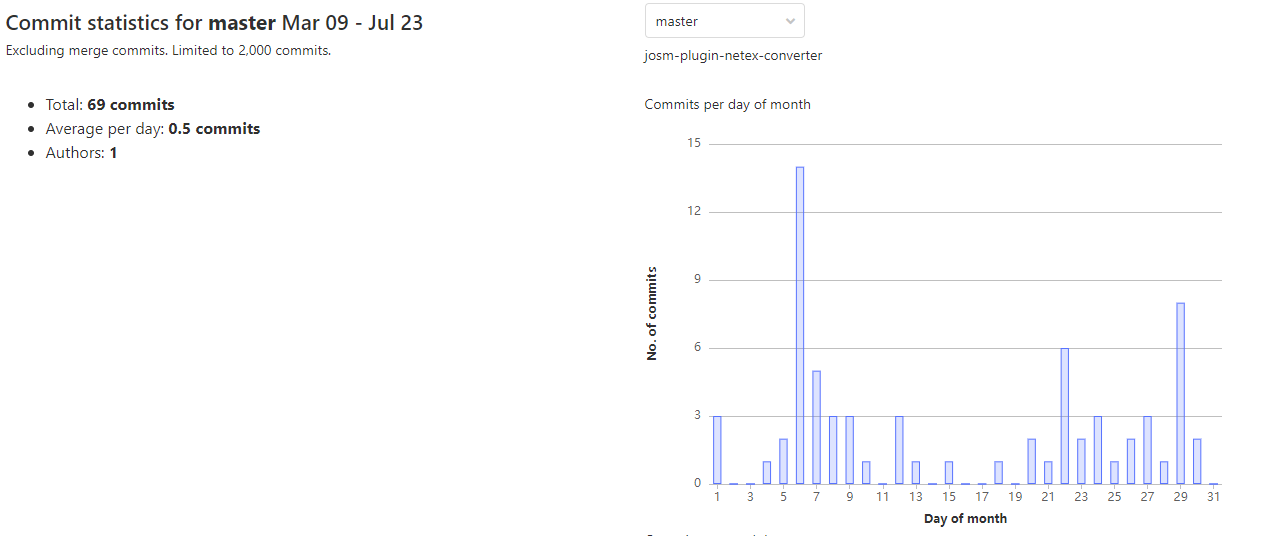
\includegraphics[width=\linewidth]{./Images/Appendices/gitlab_commit_stats.png}
	\caption{Some statistics about GitLab code commits (Commits per day are a little outdated)}
\end{figure}
\begin{figure}[H]
	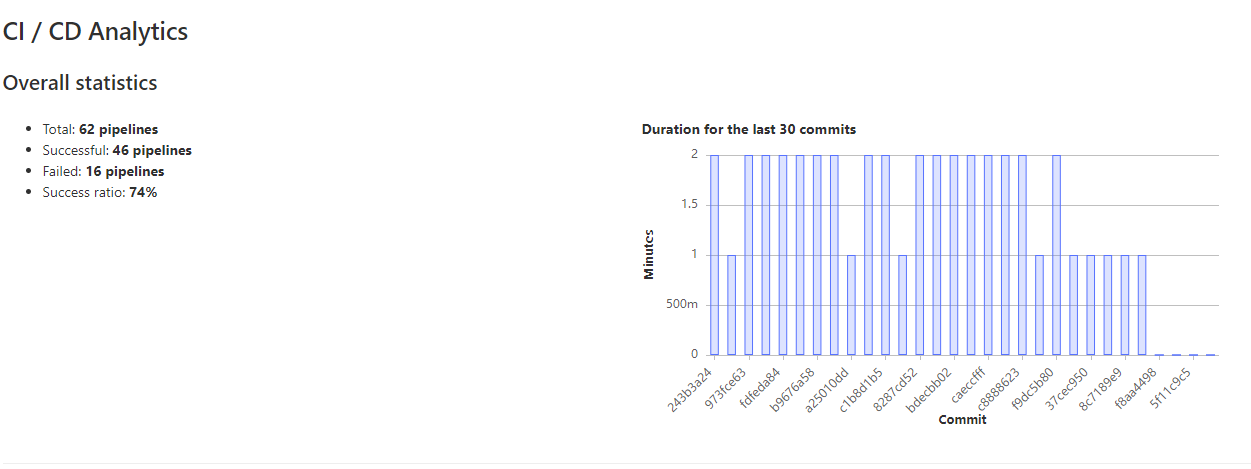
\includegraphics[width=\linewidth]{./Images/Appendices/gitlab_cicd_stats.png}
	\caption{Some statistics about GitLab CI/CD pipelines}
\end{figure}